

\tikzset{every picture/.style={line width=0.75pt}} %set default line width to 0.75pt        

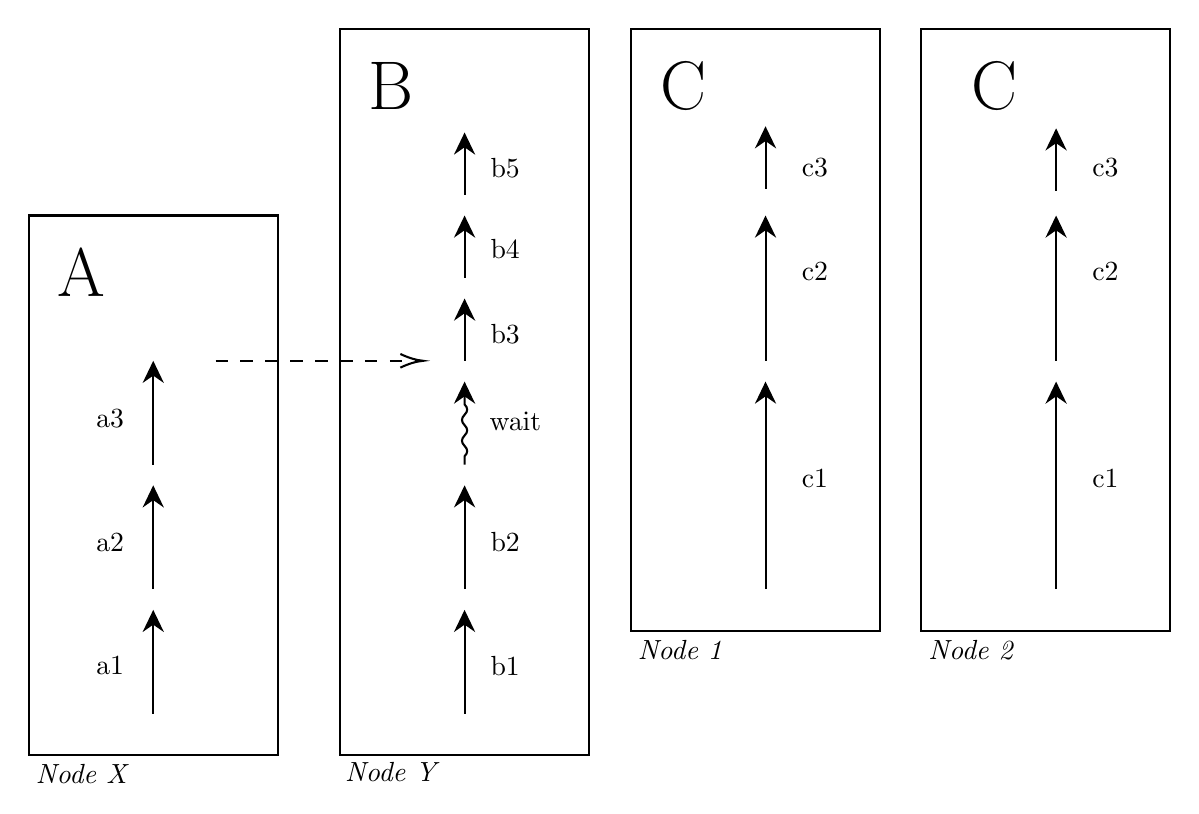
\begin{tikzpicture}[x=0.75pt,y=0.75pt,yscale=-1,xscale=1]
%uncomment if require: \path (0,413); %set diagram left start at 0, and has height of 413

%Straight Lines [id:da27430706126077264] 
\draw [color={rgb, 255:red, 0; green, 0; blue, 0 }  ,draw opacity=1 ][fill={rgb, 255:red, 255; green, 0; blue, 0 }  ,fill opacity=1 ][line width=0.75]    (80,360) -- (80,313) ;
\draw [shift={(80,310)}, rotate = 450] [fill={rgb, 255:red, 0; green, 0; blue, 0 }  ,fill opacity=1 ][line width=0.08]  [draw opacity=0] (10.72,-5.15) -- (0,0) -- (10.72,5.15) -- (7.12,0) -- cycle    ;
%Straight Lines [id:da18541775456344745] 
\draw [color={rgb, 255:red, 0; green, 0; blue, 0 }  ,draw opacity=1 ][fill={rgb, 255:red, 144; green, 19; blue, 254 }  ,fill opacity=1 ][line width=0.75]    (80,300) -- (80,253) ;
\draw [shift={(80,250)}, rotate = 450] [fill={rgb, 255:red, 0; green, 0; blue, 0 }  ,fill opacity=1 ][line width=0.08]  [draw opacity=0] (10.72,-5.15) -- (0,0) -- (10.72,5.15) -- (7.12,0) -- cycle    ;
%Straight Lines [id:da9191051295157292] 
\draw    (80,240) -- (80,193) ;
\draw [shift={(80,190)}, rotate = 450] [fill={rgb, 255:red, 0; green, 0; blue, 0 }  ][line width=0.08]  [draw opacity=0] (10.72,-5.15) -- (0,0) -- (10.72,5.15) -- (7.12,0) -- cycle    ;
%Straight Lines [id:da565354971469586] 
\draw [color={rgb, 255:red, 0; green, 0; blue, 0 }  ,draw opacity=1 ][line width=0.75]    (230,360) -- (230,313) ;
\draw [shift={(230,310)}, rotate = 450] [fill={rgb, 255:red, 0; green, 0; blue, 0 }  ,fill opacity=1 ][line width=0.08]  [draw opacity=0] (10.72,-5.15) -- (0,0) -- (10.72,5.15) -- (7.12,0) -- cycle    ;
%Straight Lines [id:da6700429327448342] 
\draw [color={rgb, 255:red, 0; green, 0; blue, 0 }  ,draw opacity=1 ][line width=0.75]    (230,300) -- (230,253) ;
\draw [shift={(230,250)}, rotate = 450] [fill={rgb, 255:red, 0; green, 0; blue, 0 }  ,fill opacity=1 ][line width=0.08]  [draw opacity=0] (10.72,-5.15) -- (0,0) -- (10.72,5.15) -- (7.12,0) -- cycle    ;
%Straight Lines [id:da28075371980457553] 
\draw [color={rgb, 255:red, 0; green, 0; blue, 0 }  ,draw opacity=1 ]   (230,190) -- (230,163) ;
\draw [shift={(230,160)}, rotate = 450] [fill={rgb, 255:red, 0; green, 0; blue, 0 }  ,fill opacity=1 ][line width=0.08]  [draw opacity=0] (10.72,-5.15) -- (0,0) -- (10.72,5.15) -- (7.12,0) -- cycle    ;
%Straight Lines [id:da9441221295165446] 
\draw [color={rgb, 255:red, 0; green, 0; blue, 0 }  ,draw opacity=1 ]   (230,150) -- (230,123) ;
\draw [shift={(230,120)}, rotate = 450] [fill={rgb, 255:red, 0; green, 0; blue, 0 }  ,fill opacity=1 ][line width=0.08]  [draw opacity=0] (10.72,-5.15) -- (0,0) -- (10.72,5.15) -- (7.12,0) -- cycle    ;
%Straight Lines [id:da3794379224544834] 
\draw [color={rgb, 255:red, 0; green, 0; blue, 0 }  ,draw opacity=1 ][line width=0.75]    (230,110) -- (230,83) ;
\draw [shift={(230,80)}, rotate = 450] [fill={rgb, 255:red, 0; green, 0; blue, 0 }  ,fill opacity=1 ][line width=0.08]  [draw opacity=0] (10.72,-5.15) -- (0,0) -- (10.72,5.15) -- (7.12,0) -- cycle    ;
%Straight Lines [id:da13857817807873274] 
\draw [color={rgb, 255:red, 0; green, 0; blue, 0 }  ,draw opacity=1 ]   (375,300) -- (375,203) ;
\draw [shift={(375,200)}, rotate = 450] [fill={rgb, 255:red, 0; green, 0; blue, 0 }  ,fill opacity=1 ][line width=0.08]  [draw opacity=0] (10.72,-5.15) -- (0,0) -- (10.72,5.15) -- (7.12,0) -- cycle    ;
%Straight Lines [id:da18881367347259226] 
\draw [color={rgb, 255:red, 0; green, 0; blue, 0 }  ,draw opacity=1 ]   (375,190) -- (375,123) ;
\draw [shift={(375,120)}, rotate = 450] [fill={rgb, 255:red, 0; green, 0; blue, 0 }  ,fill opacity=1 ][line width=0.08]  [draw opacity=0] (10.72,-5.15) -- (0,0) -- (10.72,5.15) -- (7.12,0) -- cycle    ;
%Straight Lines [id:da5578630098708864] 
\draw [color={rgb, 255:red, 0; green, 0; blue, 0 }  ,draw opacity=1 ][line width=0.75]    (375,107) -- (375,80) ;
\draw [shift={(375,77)}, rotate = 450] [fill={rgb, 255:red, 0; green, 0; blue, 0 }  ,fill opacity=1 ][line width=0.08]  [draw opacity=0] (10.72,-5.15) -- (0,0) -- (10.72,5.15) -- (7.12,0) -- cycle    ;
%Straight Lines [id:da8425704792181163] 
\draw [color={rgb, 255:red, 0; green, 0; blue, 0 }  ,draw opacity=1 ]   (515,300) -- (515,203) ;
\draw [shift={(515,200)}, rotate = 450] [fill={rgb, 255:red, 0; green, 0; blue, 0 }  ,fill opacity=1 ][line width=0.08]  [draw opacity=0] (10.72,-5.15) -- (0,0) -- (10.72,5.15) -- (7.12,0) -- cycle    ;
%Straight Lines [id:da4623771258590563] 
\draw [color={rgb, 255:red, 0; green, 0; blue, 0 }  ,draw opacity=1 ]   (515,190) -- (515,123) ;
\draw [shift={(515,120)}, rotate = 450] [fill={rgb, 255:red, 0; green, 0; blue, 0 }  ,fill opacity=1 ][line width=0.08]  [draw opacity=0] (10.72,-5.15) -- (0,0) -- (10.72,5.15) -- (7.12,0) -- cycle    ;
%Straight Lines [id:da01593649548581877] 
\draw [color={rgb, 255:red, 0; green, 0; blue, 0 }  ,draw opacity=1 ][line width=0.75]    (515,108) -- (515,81) ;
\draw [shift={(515,78)}, rotate = 450] [fill={rgb, 255:red, 0; green, 0; blue, 0 }  ,fill opacity=1 ][line width=0.08]  [draw opacity=0] (10.72,-5.15) -- (0,0) -- (10.72,5.15) -- (7.12,0) -- cycle    ;
%Straight Lines [id:da11733369284313999] 
\draw    (230,203) -- (230,211) .. controls (231.67,212.67) and (231.67,214.33) .. (230,216) .. controls (228.33,217.67) and (228.33,219.33) .. (230,221) .. controls (231.67,222.67) and (231.67,224.33) .. (230,226) .. controls (228.33,227.67) and (228.33,229.33) .. (230,231) .. controls (231.67,232.67) and (231.67,234.33) .. (230,236) -- (230,240) -- (230,240) ;
\draw [shift={(230,200)}, rotate = 90] [fill={rgb, 255:red, 0; green, 0; blue, 0 }  ][line width=0.08]  [draw opacity=0] (10.72,-5.15) -- (0,0) -- (10.72,5.15) -- (7.12,0) -- cycle    ;
%Shape: Rectangle [id:dp7566501532885672] 
\draw   (20,120) -- (140,120) -- (140,380) -- (20,380) -- cycle ;
%Shape: Rectangle [id:dp7161333832931515] 
\draw   (170,30) -- (290,30) -- (290,380) -- (170,380) -- cycle ;
%Shape: Rectangle [id:dp06857446125901545] 
\draw   (310,30) -- (430,30) -- (430,320) -- (310,320) -- cycle ;
%Shape: Rectangle [id:dp2065823399364003] 
\draw   (450,30) -- (570,30) -- (570,320) -- (450,320) -- cycle ;
%Straight Lines [id:da9709501590934354] 
\draw  [dash pattern={on 4.5pt off 4.5pt}]  (110,190) -- (208,190) ;
\draw [shift={(210,190)}, rotate = 180] [color={rgb, 255:red, 0; green, 0; blue, 0 }  ][line width=0.75]    (10.93,-3.29) .. controls (6.95,-1.4) and (3.31,-0.3) .. (0,0) .. controls (3.31,0.3) and (6.95,1.4) .. (10.93,3.29)   ;

% Text Node
\draw (45.5,147.5) node  [font=\Huge] [align=left] {A};
% Text Node
\draw (194.5,57.5) node  [font=\Huge] [align=left] {B};
% Text Node
\draw (335.5,57.5) node  [font=\Huge] [align=left] {C};
% Text Node
\draw (485.5,57.5) node  [font=\Huge] [align=left] {C};
% Text Node
\draw (254.5,219) node   [align=left] {wait};
% Text Node
\draw (391,241) node [anchor=north west][inner sep=0.75pt]   [align=left] {c1};
% Text Node
\draw (391,141) node [anchor=north west][inner sep=0.75pt]   [align=left] {c2};
% Text Node
\draw (391,91) node [anchor=north west][inner sep=0.75pt]   [align=left] {c3};
% Text Node
\draw (531,241) node [anchor=north west][inner sep=0.75pt]   [align=left] {c1};
% Text Node
\draw (531,141) node [anchor=north west][inner sep=0.75pt]   [align=left] {c2};
% Text Node
\draw (531,91) node [anchor=north west][inner sep=0.75pt]   [align=left] {c3};
% Text Node
\draw (241,331) node [anchor=north west][inner sep=0.75pt]   [align=left] {b1};
% Text Node
\draw (241,271) node [anchor=north west][inner sep=0.75pt]   [align=left] {b2};
% Text Node
\draw (241,171) node [anchor=north west][inner sep=0.75pt]   [align=left] {b3};
% Text Node
\draw (241,130) node [anchor=north west][inner sep=0.75pt]   [align=left] {b4};
% Text Node
\draw (241,91) node [anchor=north west][inner sep=0.75pt]   [align=left] {b5};
% Text Node
\draw (51,331) node [anchor=north west][inner sep=0.75pt]   [align=left] {a1};
% Text Node
\draw (51,272) node [anchor=north west][inner sep=0.75pt]   [align=left] {a2};
% Text Node
\draw (51,212) node [anchor=north west][inner sep=0.75pt]   [align=left] {a3};
% Text Node
\draw (312,323) node [anchor=north west][inner sep=0.75pt]   [align=left] {\textit{Node 1}};
% Text Node
\draw (452,323) node [anchor=north west][inner sep=0.75pt]   [align=left] {\textit{Node 2}};
% Text Node
\draw (22,383) node [anchor=north west][inner sep=0.75pt]   [align=left] {\textit{Node X}};
% Text Node
\draw (171,382) node [anchor=north west][inner sep=0.75pt]   [align=left] {\textit{Node Y}};


\end{tikzpicture}
